%%
%% This is file `skeleton.tex',
%% generated with the docstrip utility.
%%
%% The original source files were:
%%
%% nuthesis.dtx  (with options: `skeleton')
%% 

%%
%% For common degrees, you can use the class options:
%% phd, edd, ms, ma
%% phd is the default
\documentclass[print]{nuthesis}

\usepackage{graphicx}


\begin{document}
%% Start formatting the first few special pages
%% frontmatter is needed to set the page numbering correctly
\frontmatter

\title{Enabling Distributed Scientific Computing on the Campus}
\author{Derek Weitzel}
\adviser{Dr. David Swanson}
\adviserAbstract{Someone}
\major{Computer Science}
\degreemonth{May}
\degreeyear{2014}
%%
%% For most people the defaults will be correct, so they are commented
%% out. To manually set these, just uncomment and make the needed
%% changes.
%% \college{Your college}
%% \city{Your City}
%%
%% For most people the following can be changed with a class
%% option. To manually set these, just uncomment the following and
%% make the needed changes.
%% \doctype{Thesis or Dissertation}
%% \degree{Your degree}
%% \degreeabbreviation{Your degree abbr.}
%%
%% Now that we know everything we need, we can generate the title page
%% itself.
%%
\maketitle
%%
%% You have a maximum of 350 words for your abstract, which includes
%% your title, name, etc.
%%
%% Required
\begin{abstract}

\end{abstract}

%% Optional
%% \begin{copyrightpage}
%% \end{copyrightpage}

%% Optional
%% \begin{dedication}
%% \end{dedication}

%% Optional
%% \begin{acknowledgments}
%% \end{acknowledgments}

%% Optional
%% \begin{grantinfo}
%% \end{grantinfo}
%% The ToC is required
%% Uncomment these if need be

%% The ToC is required
\tableofcontents
%% Uncomment these if need be
\listoffigures
\listoftables
%%
%% ``Real'' beginning of the document.
%% mainmatter is needed to set the page numbering correctly
%%   mainmatter is needed after the ToC, (LoF, and LoT) to set the
%%   page numbering correctly for the main body
\mainmatter

%% Thesis goes here

\chapter{Introduction}








\chapter{Related Work}
\label{chapter:relatedwork}

\section{Distributed Batch Systems}


Several batch systems and grid schedulers are able to schedule tasks on execution resources.  Examples of cluster schedulers that are frequently used are PBS \cite{pbstorque}, \mbox{HTCondor} \cite{litzkow1988condor}, and SLURM \cite{yoo2003slurm}.  Each scheduler is very good at resource management within a single administrative domain.  But, each of these resource managers have very limited ability to send processing to remote resources, which are typically under a separate administrative domain.  PBS and SLURM can send jobs between clusters that run the same schedulers.  HTCondor also has the ability to send processing to other clusters running HTCondor and it can also transform jobs to the language of other schedulers such as PBS and SLURM.

Grid schedulers have become more popular as the number of resources has increased.  Examples of grid schedulers are OSGMM \cite{website:osgmm} and GlideinWMS \cite{sfiligoi2008glideinwms}.  These schedulers are able to send jobs to remote resources using grid protocols.  OSGMM performs a direct grid submission to the remote resources using the GRAM  \cite{foster1999globus} interface.  GlideinWMS also submits to the GRAM interface of the cluster, but provides an overlay of HTCondor daemons on top of remote resources.  The overlay presents a consistent HTCondor interface to the computing resources for ease of use.  


\section{Distributed Storage Access}

Distributed file systems have long had their own storage access methods.  An example of this is Hadoop \cite{white2012hadoop}, a popular distributed file and processing system.  The only method to access Hadoop storage is through the Hadoop protocol.  On the Open Science Grid, the primary access methods are through file system independent middleware such as the Storage Resource Manager (SRM) \cite{shoshani2002storage} and XRootd \cite{dorigo2005xrootd}.  They provide a translation layer from system independent grid protocols and security mechanisms to the underlying storage system, such as Hadoop.  The Storage Resource Manager (SRM) is a previously popular protocol to access remote distributed filesystems.  It is a standardized protocol that allows remote, distributed access to large storage with APIs to balance transfers among many data servers.


Beyond storage access methods are storage schedulers.  These schedulers do not define a protocol to access the storage, rather they coordinate the access.  NeST \cite{bent2002flexibility} is a software-only grid aware storage scheduler.  It supports multiple transfer protocols into a storage device, including GridFTP \cite{allcock2005globus} and NFS \cite{walsh1985overview}.  Further, it provides features such as resource discovery, storage guarantees, quality of service, and user authentication.  It is layered over a distributed filesystem to provide access to it.  NeST functions as the interface and access scheduler for a storage device.  Features such as the storage guarantees and quality of service require NeST to be the only interface into the storage device, a very rare feature in today's grid storage.  Today's storage elements, such as the 3PB storage at Nebraska, include multiple interfaces to access the storage element.  Nebraska runs at least four \cite{attebury2009hadoop} methods of accessing and modifying storage, SRM \cite{shoshani2002storage}, GridFTP, XrootD, and Fuse \cite{szeredi2010fuse} mounted Hadoop.  All of these methods are required for compatibility with different access patterns and clients.  NeST could implement each of these protocols, but it would be extremely difficult to manage the storage centrally.  For example, Fuse is mounted on all 300 worker nodes.  The GridFTP and XrootD servers run on 10's of servers, with an aggregate bandwidth of 10Gbps.  Scaling quality of service and storage allocation / enforcement across all of these access methods would likely prove impossible.



\section{Data Transfer Mechanisms}

A popular consumer transfer method, Bittorrent, has been used for data transfer in computational grids by Wei et al \cite{wei2005collaborative, wei2005scheduling, wei2007towards}.  It has been shown to improve data transfer speeds when compared to traditional source and sink transfer methods, in this case FTP \cite{postel1985file}, which is very similar in architecture to GridFTP, a grid enabled FTP protocol.  The researchers did not compare performance of the bittorrent protocol when compared to modern grid transfer techniques, such as using HTTP local caching.  Further, the authors do not test bittorrent transfers across network partitions that are common on the grid.  For example, a worker node from one cluster may not be able to communicate directly with another cluster.  Therefore, bittorrent may not work between clusters, but will work inside clusters.

Globus online \cite{foster2011globus} is a web interface for transferring files between sites and sharing data with other users.  It offers an intuitive web interface for bulk transfers between endpoints.  It only supports the gridftp \cite{allcock2005globus} transfer protocol, and requires GridFTP implementations at all endpoints.

Stork \cite{kosar2004stork} is a data placement scheduler.  It can schedule data placement and transfers to and from remote storage systems.  Stork is innovative in that it treats data transfers similar to jobs.  It will queue transfers, and checks for proper completion of the transfers.

Kangaroo \cite{thain2001kangaroo} is another storage scheduler multi-level file access system.  It allows for multiple levels of staging in order to send job output back to a storage device.  It can do this by asynchronously staging data through multiple storage devices on it's path to the destination filesystem.  The Kangaroo system only addresses output data.

\section{Data Management}

There have been previous policy frameworks for distributed storage.  These frameworks have largely been designed to move data between few large filesystems.  Therefore, the interactions are rare, but could make significant changes to the system.  In contrast, the CacheD's have frequent interactions with other agents, but each one has a minimal impact on the entire system.

Data management is different from data transfer and access in that it provides services on top of the file systems, such as meta-data storage and search capabilities.  An example of a Data management service is iRods \cite{rajasekar2010irods}.  It provides meta-data storage and querying, and rule based placements.  Further, it can handle transfers to storage resources.

DQ2 \cite{branco2008managing} and Phedex \cite{rehn2006phedex} are production transfer services for the Atlas and CMS physics experiments, respectively.  They are used to manage distributed transfers to and from sites inside the collaborations.  Additionally, they have had databases built on top of them that provide features such as combining files into datasets for easier bulk transfer management.  Both were designed for their experiments, and therefore would be very difficult to generalize for outside users.

\begin{figure}[ht!]
	\centering
	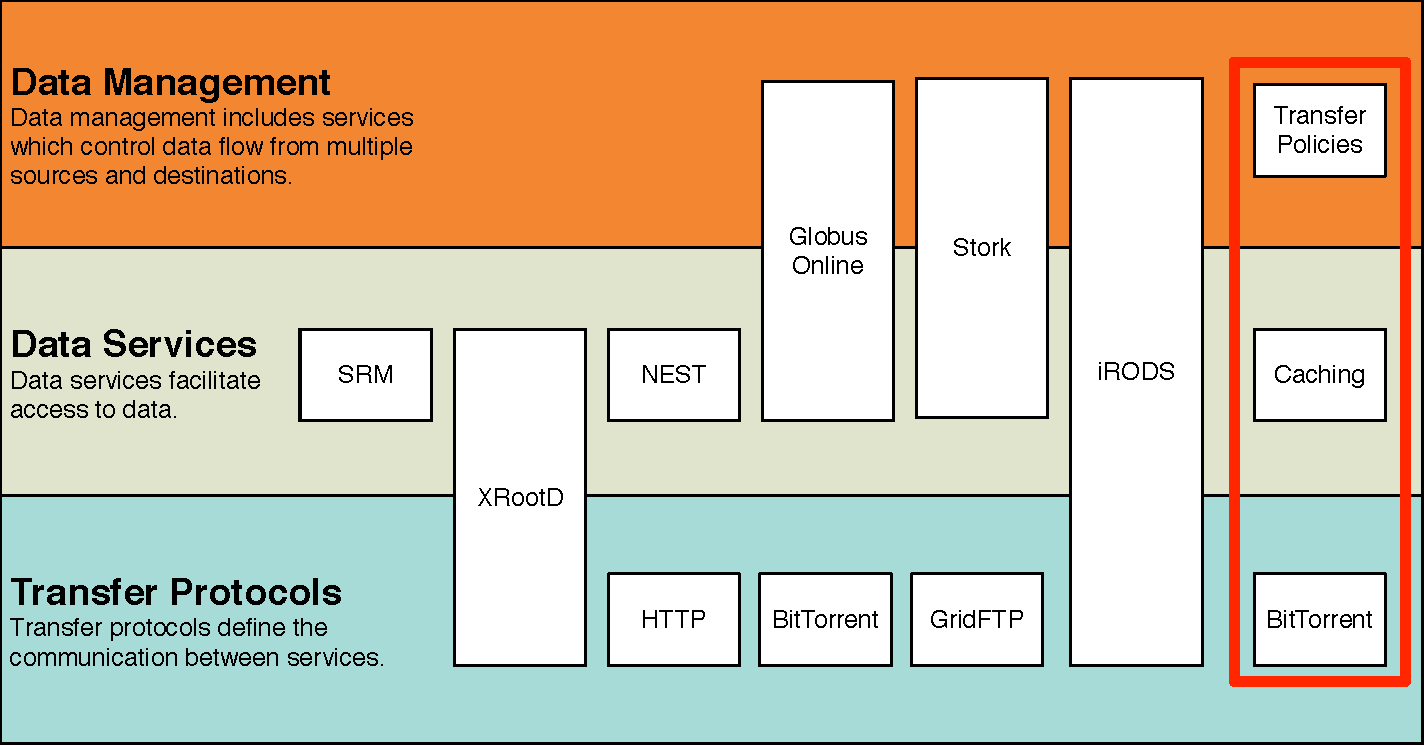
\includegraphics[width=\textwidth]{images/BackgroundStorageDiagram2.pdf}
	\caption{Background on storage technologies}
	\label{fig:backgroundstorage}
\end{figure}


\section{State of Practice in Campus Computing}
%TODO: write state of practice in campus computing





\chapter{Campus Job Distribtuion}
\label{chapter:campusjobs} 
\section{Introduction}

Campus computing is usually defined as a cluster, or a set of clusters available to researchers.  These clusters are divided either by purpose, i.e. owned by a certain group, or by hardware generations.  Users submit to a single cluster, and their jobs are eligible to run on that cluster.  I propose a framework to distribute jobs to multiple campus clusters transparently to the user.  I named the framework Bosco.  

There are many challenges for researchers on campuses with multiple, distinct clusters.  For example, a researcher may not know which cluster may run their jobs the quickest.  Or which cluster may start the jobs first.  Each of these challenges can force the researcher to make decisions that may be suboptimal and slow down their research.

Traditional cluster computing requires the user to log into the cluster and submit their processing and data there. Researchers are most comfortable on their own laptop computer.  Therefore, a submission method to enable job processing to originate from the user's laptop to be run on a remote cluster would provide a more convenient user interface.

Another challenge for researchers attempting to use these clusters is the inability to install applications.  Campus clusters only give researchers limited capabilities on the resources in order to protect the clusters' integrity.

A number of different methods have been used to distribute jobs across multiple resources.  Inside a cluster, schedulers such as HTCondor  \cite{litzkow1988condor} and PBS \cite{henderson1995job} have been used.  Neither of these schedulers have been used to submit jobs from users' laptops, a key requirement in improving the user experience.  Remote submission is heavily used in computational grids, and they use technology such as Globus \cite{foster2001globus} and UNICORE \cite{romberg2002unicore}. This remote submission requires software installation on a server inside the cluster, which requires an administrator.

Bosco \cite{weitzel2014accessing} is used to effortlessly create a remote submission endpoint on a cluster without requiring the administrator to install any software.  Bosco is a remote submission framework based upon HTCondor.  It uses the SSH \cite{ylonen2006secure} protocol to submit and monitor remotely submitted jobs.  Additionally, it performs file transfers using the same SSH connection.

Improving the user experience was a primary goal of Bosco.  I addressed the user experience by improving the interaction with the user during the installation/configuration.  Another problem area I found is when a user must debug issues with distributed software.  In order to address this, I created a traceroute \cite{mao2003towards} like utility.  The traceroute utility tests every step of the job submission process, from network access to a properly configured remote scheduler.  If an error is found at any step of the traceroute, a useful message is given to the user, including possible steps to fix the problem.




In this chapter, I will discuss the methods developed to aid in distributed scientific computing on a research campus using Bosco.  

\section{Bosco Architecture}
\label{sec:boscoarch}

% Flow of job (from picture)
% Installer improvement
% 
%TODO: Show command line

The Bosco user experience can be described in two sections: installation/configuration and running jobs.  Each of these areas was approached with the goal of improving the typical user experience for installing and running distributed computing software.

The Bosco architecture is divided into the submit host and the cluster login node.  The submit host is where the user submits their jobs and where the user interacts with the Bosco system.  The login node is the submit host for a cluster.  The login node is assumed to not be maintained by the user submitting to Bosco.  The login node has access to the local scheduler with commands such as \texttt{qsub} and \texttt{qstat} (for PBS).  

\subsection{Installation \& Configuration}
Though typically separate, Bosco combined the installation and configuration steps in order to improve the user experience.  Both are done by a single script, the \texttt{bosco\_quickstart} script that follows several steps:

\begin{enumerate}
\item Determine the platform and download the appropriate version of Bosco (supports Mac, EL5/6, Debian 6)
\item Install Bosco into the user's home directory.
\item Prompt the user for details of connecting their first cluster to Bosco.
\end{enumerate}

The script downloads the Bosco binaries from a central server to the submit host.  Bosco is installed into the user's home directory by default in order to enable non-root installations.  Connecting a cluster to the Bosco submit host requires configuring the secure connection to the cluster, and installing a small amount of software on the submit node that will be used for job submission and job status checks.

The installation on the user's laptop and on the remote cluster do not require administrator access.  All files and applications are installed in the user's directories.

I have also created a native installer, a PKG, for the Mac version of Bosco.  It is distributed in an Apple Disk Image (DMG) for consistency with other Mac software.  Unlike the Linux installer, it does not automatically configure a cluster at first installation.


\subsection{Running Jobs}

The image shown in Figure \ref{fig:archgraph1} shows the architecture of job submissions of a Bosco submit node.  Job submissions are done from the Bosco submit host, which in turn submit to the connected cluster login node.  

\begin{sidewaysfigure}[h!t]
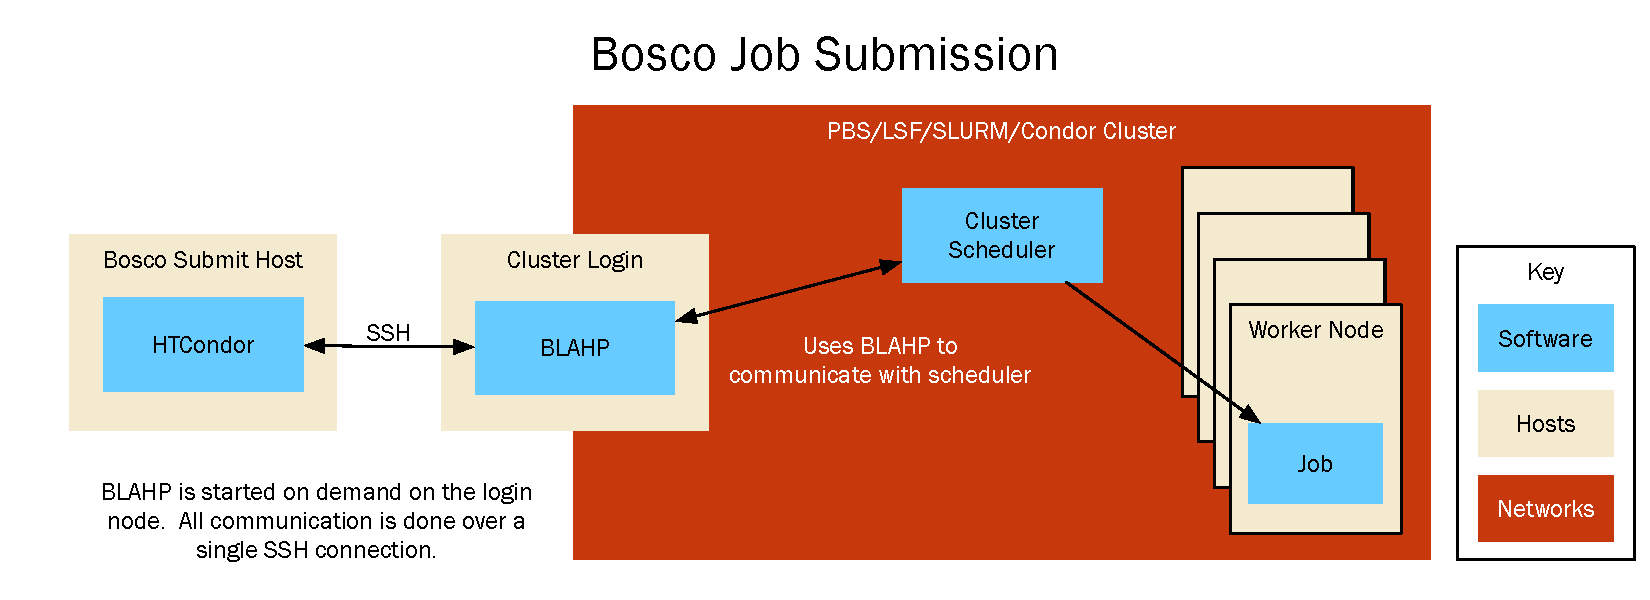
\includegraphics[width=\textwidth]{images/ArchitectureGraph1}
\caption{Bosco Architecture}
\label{fig:archgraph1}
\end{sidewaysfigure}
\afterpage{\clearpage}

First, the Bosco submit node connects to the login node over an SSH connection and creates the forwarded SSH tunnel back to the submit node, which is used for file transfer.  SSH was chosen as the protocol, since it is used nearly universally for cluster access.  It creates the forwarded SSH tunnel in order to minimize the number of connections between the Bosco submit host and the login node.  By reusing the same SSH connection, I reduce the number of SSH logins to one.  Further, the number of connections is not dependent on the number of jobs, as Bosco will reuse the same connection for all jobs submitted to a cluster.  Minimizing the number of connections to a login node is important since many login nodes include firewall rules to slow down brute force SSH logins that block frequent successive SSH connections.  The Bosco submit host does not require any open ports in a firewall, only outgoing connections to a remote login node's SSH port.

%    Jobs are submitted to Bosco, which then submits over ssh to the remote cluster.  Input files are transferred over the SSH connection as well.  Bosco then monitors and reports the status of the job on the remote cluster as idle, running, or completed.  Once the job is completed, Bosco will transfer output files back to the submit host.


Next, Bosco checks for the necessary installed software on the login node, and starts the BLAHP \cite{blahp} daemon that will communicate with the scheduler on the login node.  The BLAHP daemon on the login node starts the file transfer daemon to connect back to the submit host through a forwarded SSH tunnel that Bosco created.  The transfer daemon creates and transfers the job sandbox to the login node.  The transfer to the login node is performed by HTCondor's fault tolerant file transfer mechanisms and are entirely encrypted over the SSH connection.  Authentication between the login node and the Bosco submit host is performed by a shared secret that was previously sent over the SSH connection to the BLAHP daemon.

After the files have been transferred, Bosco sends the job's submission ClassAd \cite{raman1998matchmaking} to the BLAHP daemon to translate to the local site's scheduler language.  The BLAHP supports PBS \cite{computing2013torque}, LSF \cite{computinglsf}, SGE \cite{gentzsch2001sun}, Slurm \cite{yoo2003slurm}, and HTCondor schedulers.  The BLAHP creates the submission file, and submits it to the cluster's scheduler.  Bosco periodically polls the BLAHP over the SSH connection for the status of the job.  Once the job is detected to have been completed, the BLAHP starts HTCondor's transfer daemon to transfer the output sandbox back to the submitter machine.

\begin{figure}[h!t]
	\centering
	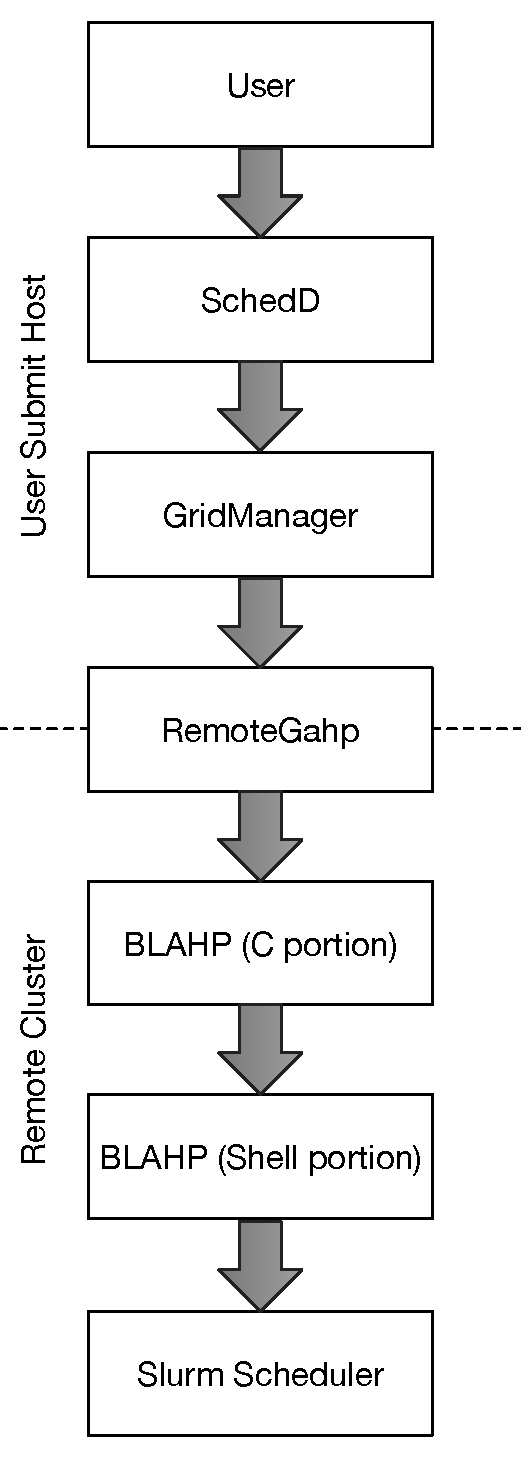
\includegraphics[width=0.3\textwidth]{images/JobSubmitFlow.pdf}
	\caption{Bosco Job Submission Flow From Submission Host to Remote Cluster}
	\label{fig:boscojobsubmitflow}
\end{figure}

Figure \ref{fig:boscojobsubmitflow} shows the job flow from the user to the Slurm scheduler on the remote cluster.  As you can see it goes through six daemons before reaching the cluster scheduler.  The HTCondor job manager agent (SchedD) accepts the user's jobs, acting as an agent which will attempt to execute the job.  HTCondor's grid interface daemon (GridManager) is spawned by the SchedD in order to service the Bosco job.  The RemoteGahp (Grid Ascii Helper Protocol) starts the SSH tunnel between the user submit host and the cluster.  The BLAHP (C portion) interprets the job requirements, and executes the BLAHP (shell portion) which translates the requirements into the local scheduler language.  Finally, the BLAHP submits the jobs to the Slurm Scheduler.


Bosco has two modes of job submission:
\begin{enumerate}
	\item \textbf{Direct} -- A single job on the Bosco submit host corresponds to a single job on the remote cluster.  Each job is submitted individually to the remote cluster's scheduling system.  This method is the simplest to run and imposes no special requirements on the submit machine.
	\item \textbf{Glidein} -- Bosco submits many pilot jobs to the remote cluster using the direct method.  But each of the pilots can service multiple user-submitted jobs from the Bosco submit host.  This method minimizes the overhead on the remote cluster since Bosco is not submitting many jobs through the cluster scheduler.  The glidein method requires that the Bosco submit host can be contacted from the remote cluster worker nodes. \label{sec:glidein}  The glidein submission method is based off of previously written software such as the Campus Factory \cite{weitzel2011campus}.
\end{enumerate}

The two modes of job submission allow users to optimize for their environment.  If they are running many short identical jobs (which is frequent in high throughput computing), then the glidein method is ideal for them.  If they are running fewer, longer, and possibly unique requirement jobs; then the direct submission method would work best.  Most users start with the direct method then graduate to glidein once they become accustomed to submitting batch jobs.

Bosco's fault tolerance is in its handling of the remote cluster.  For example, if the user's computer loses connection with the remote cluster due to network issues, or even if the user suspends their laptop, Bosco will place the jobs on hold.  Although no new jobs will be submitted to the remote cluster, jobs that were already submitted will continue to run.  Further, when Bosco re-establishes a connection to the remote cluster, Bosco will check the status of already submitted jobs.  It will then bring back any output data from any jobs that have completed and continue to submit jobs to the remote scheduler.

\subsection{Improving User Experience}


In order to improve the user experience at each step of the job process, extra effort has been given to provide useful error messages in case of failures.  For example, HTCondor was modified to relay the standard error for any commands sent to the BLAHP daemon, as useful debugging information is available there.  

\label{sec:boscotraceroute}

Also, an additional traceroute was created to test each step of the job submission process, including:

\begin{description}
\item[SSH connection to the remote login host:]  Tests network connection, login host availability, and passwordless SSH setup.
\item[Job submission to the Bosco submit host:]  Tests Bosco daemon availability and Bosco submit host file system availability.
\item[Job submission to the remote login host:]  Tests the remote scheduler availability, remote cluster software setup, input file transfer, and cluster file system availability.
\item[Job completion and status update from login host:]  Tests Bosco status check process and output file transfer.
\end{description}

The traceroute is very useful for debugging issues with a Bosco installation.  It is designed to test each step in the job execution life cycle and give meaningful error messages and possible solutions.

\section{Load Balanced Access to Computational Resources}

Bosco is used in conjunction with the Campus Factory \cite{website:campusfactory}, which is described in full in my Master's thesis \cite{weitzel2011campus}.  The Campus Factory submits pilot jobs to remote clusters to create an overlay that provides a consistent interface to the resources.  The campus factory submits to multiple Bosco endpoints simultaneously, load balancing between them by keeping idle jobs (constant pressure) on all clusters.

Submission via the Bosco framework is done using the HTCondor submit syntax.  When an idle user job is detected by the Campus Factory, it begins to submit glideins to all Bosco endpoints simultaneously.  The Campus Factory maintains idle glideins on each of the endpoints until the user's jobs have completed.  The jobs run on any resources that become available.


\section{BoscoR: Extending R from the desktop to the Grid}

As a case study of improving the user experience when using Bosco and distributed computing, I created BoscoR, an interface to Bosco from the R statistical programming language.  The following was published as:

\bibentry{weitzelboscor}

\subsection{Introduction}
Usage of the R language \cite{team2012r} by data miners has grown much faster than any other programming language \cite{rexer2013, KDnuggets2013}.  Data mining requires computational resources, sometimes more computational resources than can be provided by their desktop computer.  In a recent study of data scientists \cite{rexer2013}, ``Available computing power'' was the second most common problem for big data analysis.  In addition, the respondents stated that distributed or parallel processing was the least common solution to their big data needs.  This could be attributed to the difficulty of processing data with the R language on distributed resources, a challenge I set out to solve with BoscoR.

A reason that distributed computing is not seen as a popular solution to big data processing is that scientists are more familiar processing on their desktop than in a cluster environment.  R is typically used by people that have not used distributed computing before and do most of their analysis on their local systems with integrated development environments (IDE) such as RStudio \cite{racine2012rstudio}.  Users are unaccustomed to the traditional distributed computing model of batch processing in which there is no interactive access to the running processes.

Though researchers may not have experience with distributed computing, most have computational resources available to them, either locally provided by their institution or university, or through national cyberinfrastructure such as the OSG \cite{pordes2007open} or XSEDE \cite{xsede}.



In this section, I will describe GridR \cite{wegener2007gridr}, an R library used to interact with the Bosco framework.  In section \ref{sec:boscorimplementation}, I describe how I combined these two components to create a fault-tolerant framework that provides a positive user experience.  Next, in Section \ref{sec:boscorresults}, I discuss preferred submission methods based on the length of the R function, and show I results from numerous test runs against a production cluster.  Finally, I offer some conclusions and future work.

\subsection{Background}
BoscoR is primarily made up of two components, Bosco and GridR.  Bosco provides a simple setup interface to the remote batch system, and it provides fault tolerance for job submission and file transfers.  GridR provides a user interface to create and initiate remote processing.


\subsection{GridR}
% Overview of parallel libraries
Many parallel libraries are available for R.  Most focus on managing the R processing on a single server such as the \texttt{parallel} package \cite{rparallelpackage}.  The \texttt{parallel} package comes bundled with R and provides for single machine parallelism.  Parallelism is done by using variations of the R function \texttt{lapply}.  A simplified definition of \texttt{lapply} is shown in Figure \ref{lst:lapply}.  \texttt{lapply} is the basis for nearly all parallel libraries in R.  

\begin{figure}[h!t]
\begin{framed}
\texttt{lapply}(\textbf{X}, \textbf{FUN}, \textbf{\ldots}):
\begin{description}
\item[\textbf{X}] a vector (atomic or list) or an expression object.
\item[\textbf{FUN}] the function to be applied to each element of X
\item[\textbf{\ldots}] optional arguments to FUN.
\item[Returns] list of the same length as X, each element of which is the result of applying FUN to the corresponding element of X.
\end{description}
\end{framed}

\centering
\captionsetup{justification=centering}
\caption{Function Definition of \texttt{lapply}}
\label{lst:lapply}
\end{figure}

The \texttt{lapply} function is ideally suited for high throughput computing.  There is no communication between executions of the function on the input array.  The input vector can be easily partitioned in order to split the execution across multiple resources.  It is because of these reasons that most parallel applications use the \texttt{lapply} model to provide parallelism.  Examples are the parallel package which defines the functions \texttt{mcapply} (multi-core apply) and \texttt{parapply} (parallel apply). In the \texttt{parallel} package, calling \texttt{mcapply} causes R to fork a process that will execute the function \textbf{FUN} on each element in the input vector.  A similar process happens when calling \texttt{parapply}. 

Another built-in parallelization package is Simple Network of Workstations (snow) \cite{rlangsnow}.  Snow allows for multiple computers to organize and execute parallel processing of data.  The computers communicate over regular network sockets or using MPI \cite{gropp1999using}.  This allows for multiple computers inside the same cluster to process data.  Snow also has built-in \texttt{lapply} style functionality.

GridR also follows this \texttt{lapply} model for parallelization.  It uses a function called \texttt{grid.apply}, which will apply a function to every element of an input vector, similar to \texttt{lapply}.  Instead of forking a process like \texttt{mcapply}, it compiles the input data and function, and submits the execution to a grid endpoint.

GridR was originally written for use with data analysis in ACGT clinico-genomics trials \cite{wegener2007gridr}.  It was written with the capability to submit with a limited set of grid protocols, some of which are no longer supported.  Further, GridR made assumptions of the remote resources.  These assumptions were:

\begin{itemize}
\item R is installed on all of the worker nodes.
\item The R binaries are in the same location on all of the remote resources.
\item The GridR package is installed on all of the remote resources.
\end{itemize}

All of these assumptions cannot be met on modern grid resources.  Applications cannot assume that a (non-standard) processing tool, such as R, is installed on every computer or   that it is installed at exactly the same location on all clusters in the grid.  Modifications were made to GridR to erase these assumptions, as well as to adapt it to submit to Bosco.

\subsection{Implementation}
\label{sec:boscorimplementation}

% \begin{itemize}
% \item Combining Bosco with GridR improves usability dramatically for R users.
% \item Modify GridR in order to submit to local bosco
% \item Improve scalability and fault tolerance of GridR
% \item Downloads appropriate version of R from a central repository.  Caches the R installation if available (both at the file system level, and the R level).
% \end{itemize}

Bosco is designed to run on resources that are not controlled by the submitting user.  Further, it is designed to run on resources without any conditions as to what is installed.  In order to operate under these assumptions, Bosco must bootstrap itself by bringing in all the libraries and dependencies required to operate.  Therefore, BoscoR must run under these same assumptions.

GridR was modified to submit to Bosco.  The input generation of GridR is shown in Figure \ref{fig:gridrinput}.  When a user or script calls \texttt{grid.apply}, GridR compiles the input function and input data into a R data file, which can be read later by another R process.  GridR handles function dependencies by using R's dependency detection and compiles any functions that may be required into the input.  

\begin{figure}[h!t]
\centering
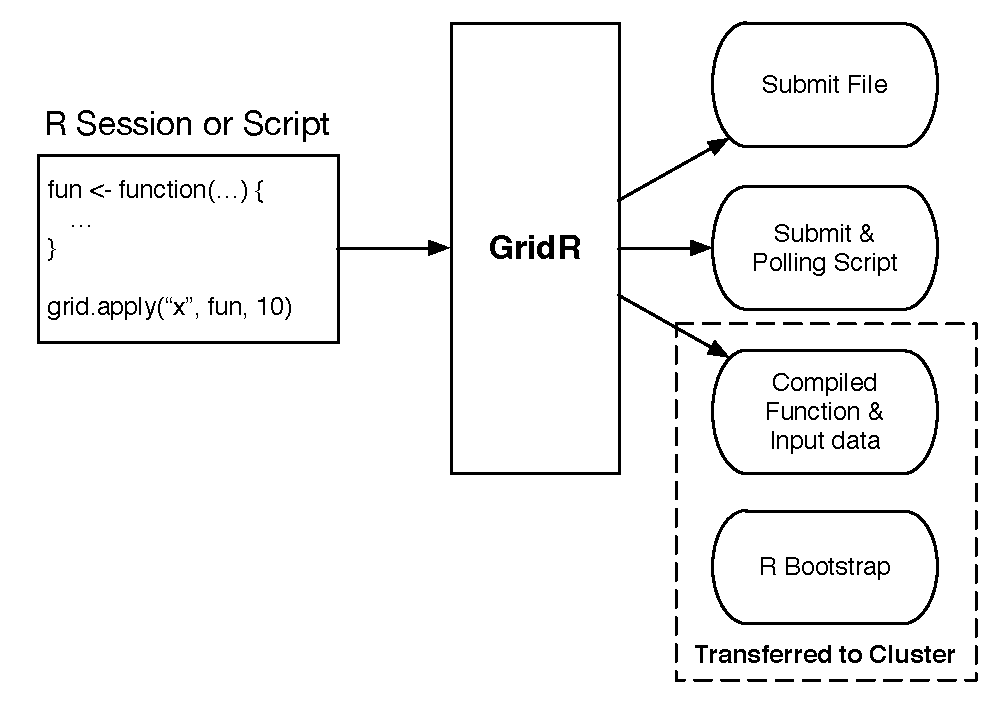
\includegraphics[width=\textwidth]{BoscoRImages/InputDiagram.pdf}
\caption{GridR Input Generation}
\label{fig:gridrinput}
\end{figure}

GridR was modified to first create a submit file which will be submitted to the local system where Bosco is installed.  The submit file explicitly lists the input files and the expected output file, all of which will be transferred by Bosco.  The input files, as shown in Figure \ref{fig:gridrinput}, are the compiled function and input data and a bootstrap executable.  The output file contains the return value from the executed function.

The submit and polling script is executed by GridR after forking a new R process.  This is a lightweight process that submits the Bosco submission script and watches for any errors.  If the input function is executed many times by many separate jobs, the polling script will aggregate the results as they are returned to the submit node into a vector that will be returned to the user.  

\subsection{Bootstrap}
\label{sec:boscorbootstrap}

Since Bosco cannot make assumptions as to what is installed on the remote cluster, neither can BoscoR.  Therefore, GridR was modified to detect, and if necessary install, R on the remote system.  This was performed by a bootstrap process.

In the GridR generated submit file, the listed executable to run on the remote system is not R, but the bootstrap executable.  The bootstrap executable detects if R is installed on the remote system.  If it is installed, it simply executes the user defined function against the input data.  If R is not installed, the bootstrap downloads the appropriate version of R for the remote operating system.  The supported platforms are identical to Bosco's: CentOS 5/6 and Debian 6/7.  R is downloaded from a central server operated by the OSG's Grid Operations Center \cite{osgoperations}.  

The bootstrap executable installs R in a shared directory.  By utilizing a shared directory, subsequent GridR jobs may use the same R installation.  Several bootstrap jobs could start at once on a remote cluster, so a simple transactional file locking mechanism was devised so only a single bootstrap executable on a cluster will download and install for the entire cluster if a shared filesystem is available.  If a shared filesystem is not available for installation, R is installed in a temporary directory that is removed upon job completion.

\subsection{Running on the Open Science Grid}

Submitting to the Open Science Grid (OSG) is done by direct submission.  The OSG hosts access nodes which can be used to submit to resources on the grid.

Most OSG sites do not have shared directories for grid users.  Therefore, the bootstrap script must install R on every node in a temporary directory.  In order to optimize the R installation, the bootstrap script utilizes the HTTP forward proxy infrastructure \cite{garzoglio2012supporting} available on the OSG to minimize requests to the central hosting server.


\subsection{Results}
\label{sec:boscorresults}

The results section is broken into two categories, results from user feedback and results from experimental runs on a production cluster as well as the OSG.

A primary goal with BoscoR was to improve the user experience of using R on distributed resources. After acquiring a few users, I received feedback on how BoscoR could be improved.  The improvements to GridR and the integration with Bosco made working with campus or institutional resources much better.  In this section I will describe the improvements.

\subsubsection{User-Provided Packages}

Many users require additional packages to be installed before their function can execute.  It was assumed that most of these packages would be in the major R package repositories, such as the Comprehensive R Archive Network (CRAN) \cite{cran}.  If the package is in CRAN, the user-provided function can install the package.  After receiving user feedback, it was found that not all desired packages are available in CRAN.  A modification to both the submit file and the bootstrap executable was designed to install such packages.

In order to install a user-provided package, it first needs to be transferred to the remote cluster.  This is done by including the package in the list of input files to be transferred by Bosco for each job.  Additionally, the packages should be installed before the user function is executed on the remote resources.  This required modification to the bootstrap executable in order to install the packages after installing R, but before executing the user's function on the input data.

\subsubsection{Quick Jobs}
Since the GridR interface only provides for a single function to execute against the input data, it was assumed that the function would be a time-consuming data-processing function.  Therefore, the overhead Bosco introduces would not significantly affect the performance of the executions.  After receiving feedback from users, it was determined that the more common use case is to use smaller functions that could execute in seconds or minutes.  In order to accommodate shorter jobs, a modification to the GridR generated submit script was required.

In this case, I modified the submit file so that Bosco would use the glidein method of job submission.  Using the glidein job submission method, the shorter jobs can be executed much more quickly, one after another, reusing the same resources.  Additionally, this saves the remote cluster scheduler from scheduling many small jobs which can cause issues in many HPC schedulers.


\subsection{Performance Results}

\subsubsection{Experimental setup}  

In order to test BoscoR, I have to simulate a R workload.  I simulate a workload with varying lengths of the executed functions.  This simulates a variety of workloads that I have seen from users.  As noted before, I assumed that the functions would be long-running data processing.  But, I learned that users were instead submitting short functions to be executed quickly.  I varied the length of function from one second to 30 minutes.  To verify my solution to quick jobs, I tested different job lengths using both the direct and glidein submission method.

To execute the test jobs, I used the production cluster, Tusker, at the University of Nebraska -- Lincoln Holland Computing Center.  This cluster is composed of 106 nodes, each with 64 cores, for a total of 6,784 cores.  The cluster has numerous users that are submitting to the central Slurm \cite{yoo2003slurm} scheduler.  The cluster traditionally runs at $>$90\% utilization, with dozens of users jobs fair sharing the resources.  The Slurm scheduler is a HPC orientated scheduler that matches submitted jobs to resources.  Fair share scheduling is used on Tusker;  each group has equal priority with all others, therefore allowing the maximum number of users to run on the resources.

Tusker is utilized enough that the jobs would be competing against other users' jobs for available resources, and therefore not all submitted GridR functions would be able to execute simultaneously.  I believe this best represents most clusters, which are typically highly utilized by many researchers.  It is plausible that a cluster could be so highly utilized that no user jobs could be executed. The other extreme could also be true: enough resources are available for all submitted jobs to be executed immediately.  I found that Tusker utilization is somewhere between these two extremes.  It is capable of running many, but not all, jobs submitted to it immediately.  The rest will execute as resources become available.

For testing, I submitted 1000 GridR jobs per test run. 1000 jobs was chosen as a reasonable representation of workflows I have seen when helping users of GridR.  They typically submit many jobs, sometimes reaching into the thousands.  The goal was to submit more jobs than could be run instantly by the remote cluster, but not so many that gathering repeated testing data would be impossibly time consuming.

\subsubsection{Direct submission}
Direct submission is defined as submission using Bosco's direct submission method.  In GridR, the library is initialized with the argument \texttt{service="bosco.direct"}.  When this setting is used, GridR generates submission scripts that use Bosco's default routing mechanism to submit to a single cluster.  The GridR functions are submitted as jobs directly to Tusker's Slurm scheduler.

\begin{figure}[h!t]
\centering
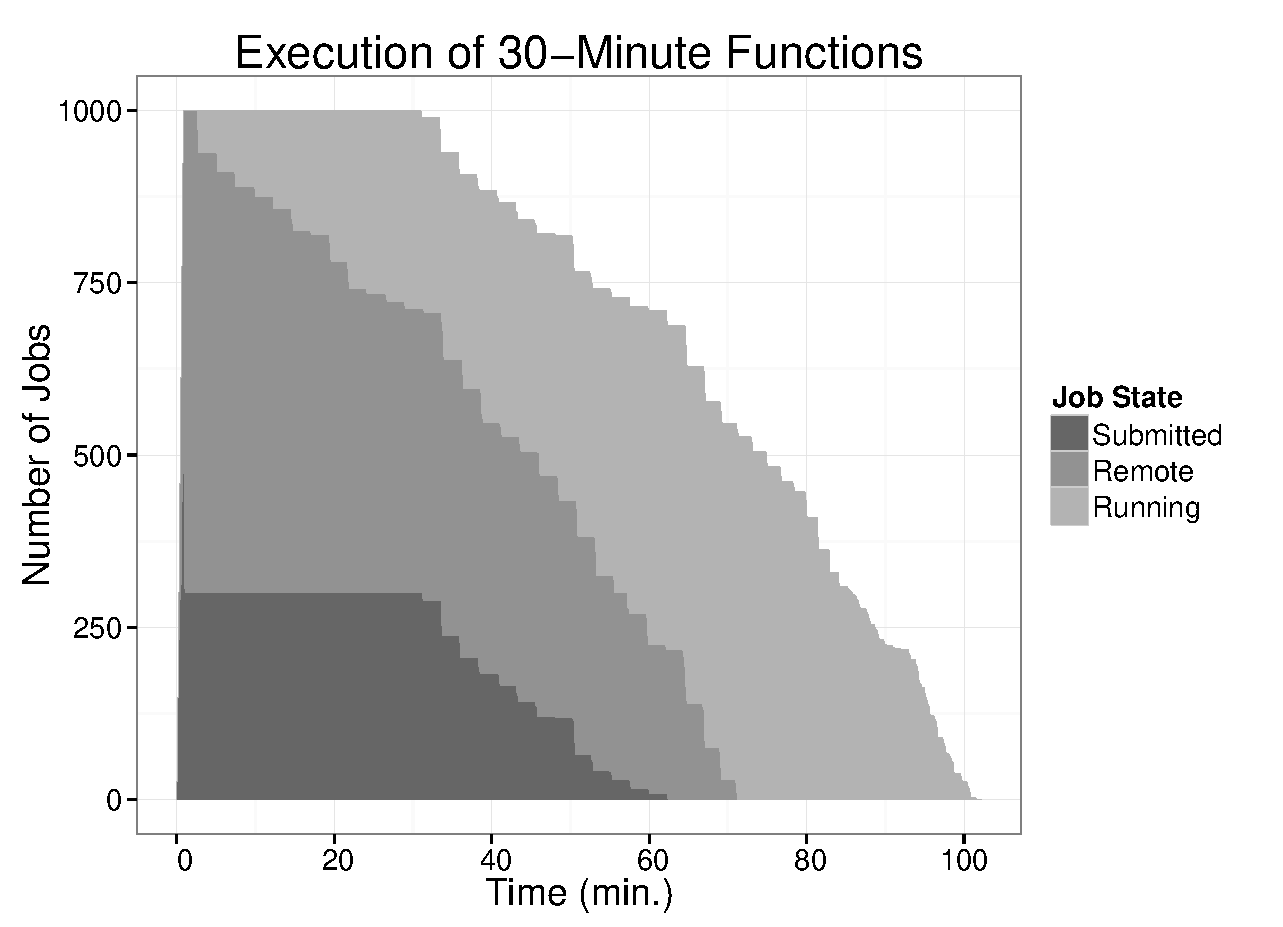
\includegraphics[width=\textwidth]{BoscoRImages/30minplot-color.pdf}

\caption{Direct Submission}
\label{fig:directsubmit}
\end{figure}

A timeline of the GridR submissions to Bosco is shown in Figure \ref{fig:directsubmit}.  The submitted jobs are jobs which are submitted locally, but not yet submitted to the remote scheduler.  Remote represents the jobs which are submitted to the remote Slurm scheduler.  The submission to the remote scheduler is very rapid.  Bosco is able to submit 700 jobs, the limit in this implementation to submit at a single time, within a minute.  Slurm is able to rapidly begin executing many, but not all, of the submitted jobs.  Bosco maintains constant pressure in the form of idle jobs in case resources become available on the cluster.  You will notice the straight line in the number of submitted jobs which dips after 30 minutes.  At 30 minutes the first jobs begin to complete and Bosco begins to submit more jobs to the cluster, attempting to always keep the maximum of 700 jobs either idle or running on the remote cluster.  In this workflow, all 1000 30 minute jobs finish in just over 100 minutes.

The Open Science Grid runs use the direct submission method as well.  But, since the OSG access nodes run HTCondor, the jobs are capable of starting much quicker after being submitted to the remote resource.  In this way, the OSG provides the best of both the direct and glidein approaches.  It is simple to setup like any direct submission method.  And as with the glidein submission method, the jobs start quickly on the remote resource.

The OSG direct submission presents different failure modes than a traditional HPC cluster.  For example, in one of our experimental runs with 1 second jobs, a single job took over 30 minutes to complete.  The issue with this particular job was that the job was matched to a single node that was misconfigured.  In this case, the job eventually finished after being matched to a different node.  The OSG may not be an ideal solution for short executions of GridR functions.

\subsubsection{Glidein}
Glidein submissions use a pilot that is submitted directly to the Slurm scheduler.  Once the pilot starts, it calls back to the submission node to request work.  This method allows multiple jobs to run within the same Slurm job, independent of the cluster's scheduler.  

\begin{figure}[h!t]
\centering
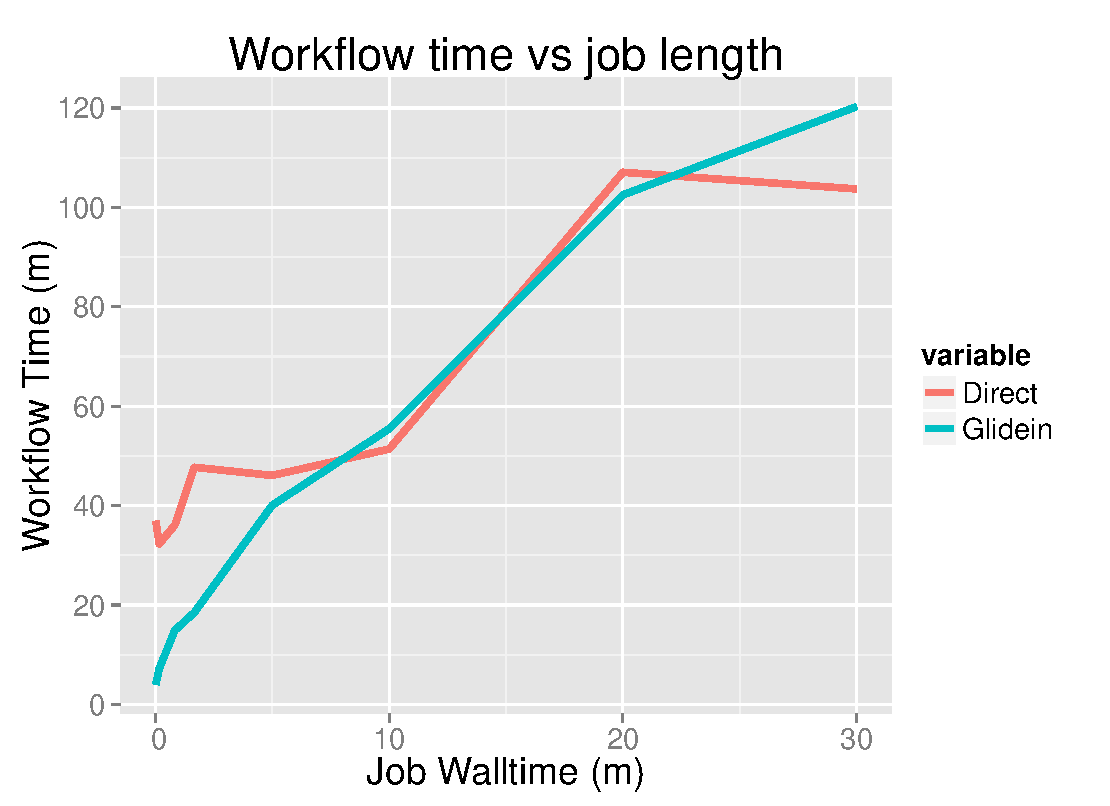
\includegraphics[width=\textwidth]{BoscoRImages/ComparisonPlot.pdf}
\caption{Comparison of submission methods}
\label{fig:comparesubmit}
\end{figure}

Comparing the direct submission to the glidein submission is shown in Figure \ref{fig:comparesubmit}  As you can see, for longer jobs, direct and glidein submission methods have approximately similar workflow runtimes.  But, for short jobs, glidein has significantly shorter workflow runtimes.  This can be attributed to the advantages of using a high throughput scheduler over a high performance scheduler.

Bosco is built on top of HTCondor.  HTCondor is a very efficient high throughput scheduler that can quickly start the execution of jobs upon available resources.  Since many R workflows are designed to run a short function upon a large amount of data, HTCondor is a good fit.  By submitting HTCondor pilots to the remote scheduler, Bosco is able to utilize its strength of running many small jobs quickly, resulting in a shorter workflow completion time for shorter jobs.

\begin{figure}[h!t]
\centering
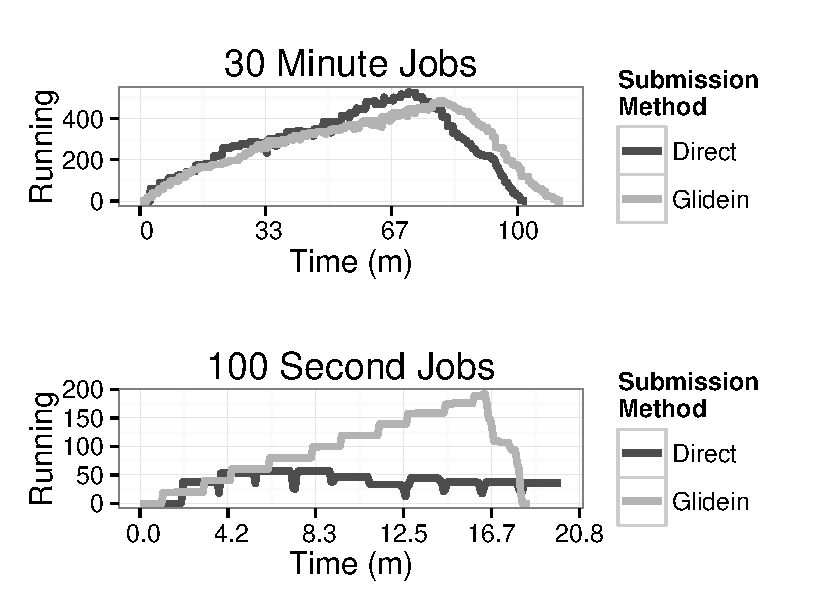
\includegraphics[width=\textwidth]{BoscoRImages/NumberRunning.pdf}

\caption{Number of simultaneously running jobs}
\label{fig:runningjobs}
\end{figure}

Figure \ref{fig:runningjobs} illustrates how the glidein submission method is superior to the direct submission method for short jobs, and why both methods are roughly equivalent for longer jobs.  For longer jobs, you can see that both glidein and direct submission methods start jobs at nearly equal rates.  The variation is relatively small, and could be explained by variations in the available resources at the time of running the experiments. 

For the shorter 100 second jobs the start rate begins nearly the same, but then Bosco and Slurm are unable to sustain the job start rate.  Since the jobs only run for 100 seconds the overhead from Bosco submission and Slurm starting the jobs becomes a bottleneck.  Bosco is only able to sustain roughly 50 jobs running on the cluster.  On the other hand, the glidein submission method continues to grow in the number of jobs running.  This is due to eliminating the Bosco submission overhead, as well as the Slurm scheduling overhead.  Instead, the glidein method is utilizing the much more efficient HTCondor scheduler, which is able to start jobs much faster than the Slurm scheduler.  I can conclude that the glidein submission method results in a shorter total workflow execution time for shorter R functions.


\subsection{Conclusion}

BoscoR is a framework to execute R functions on distributed resources.  It is a simple method for users to distribute processing to remote resources.  BoscoR incorporated user feedback in order to improve the framework.

As with any complicated system, many parameters can be varied in order to obtain different results.  For example:
\begin{itemize}
\item Resource contention may be high which could cause the cluster not to start any GridR jobs.
\item Resource contention may be low, which would cause Slurm to start all submitted jobs immediately.
\item The number of glideins submitted in a batch could be varied in order to optimize the start rate for a particular cluster.  Any lower and it would slow job starts, increasing the workflow run time for both short and long jobs.  Any higher, and it could overwhelm the remote scheduler.
\end{itemize}

I chose reasonable values for these parameters that an end user may use.  In the future I will tune these parameters automatically using the feedback provided by Bosco.  Although Bosco and the bootstrap process significantly improved the fault tolerance of GridR, further fault tolerance testing and development is needed to provide a positive user experience when running on national infrastructure such as the OSG.

During follow up interviews with users after using BoscoR, I received many positive reviews of the framework.  Improving the user experience of using R on distributed resources was a primary goal of BoscoR.  One example of a positive review was from a Micro-Biology researcher from the University of Wisconsin:
\begin{quote}
I have a huge set of data, which I have to split into pieces to be handled by each node.  This is something I can do with the "grid.apply" function. This reduces the submit time from several hours, to several seconds... it is a  phenomenal improvement. This will greatly increase my use of grid computing, as right now, I only use grid computing when I have no other choice.
\end{quote}

The experimental testing I ran showed that glidein submission method is significantly better at running short R functions than the direct submission method.  At longer job runtimes, the difference between direct and glidein submission to remote resources is negligible.






\section{Conclusion}

Bosco and the Campus Factory combine to make an easy to use framework that can distribute jobs to many computational clusters on a campus.  Users are able to effectively distribute their processing to multiple clusters using this framework.  In this section, I showed that Bosco transparently and effectively distributes computational jobs across multiple clusters on a campus, while maintaining simple usage for users.

Using Bosco as a foundation, I was able to create an interface from the R programming language called BoscoR.  This interface proved very simple for users to use.  

During the evaluation of BoscoR, I confirmed the suspicions that the direct submission method is slower for quick jobs than the glidein submission method.  But, for longer jobs, there is almost no difference between direct and glidein jobs.

Bosco's usage has increased since I originally published the Bosco paper.  For example, it is heavily used by the University of Chicago in order to submit OSG processing to opportunistic resources around the country.  They find Bosco useful since it does not require the installation of any software on the remote cluster.

Additionally, the CMS experiment has used Bosco to access opportunistic resources around the world, and has published many papers on the subject \cite{hufnagelcmsopportunistic, piperovoperationalchep15, wagner2013using, kreuzer2014opportunistic}.

If the user's workflow requires significant data, it may be inefficient to use Bosco's transfer mechanisms which are bottlenecked by the transfer speed of the Bosco submit host.  It is expected that large datasets will not be an efficient use of Bosco.  Therefore, I will introduce a framework to efficiently transfer data in Chapter \ref{chapter:campusdatadistribution} that will complement Bosco's overlay network.




In this chapter I will discuss Bosco.

\chapter{Campus Storage Access}
In this chapter I will discuss
\label{chapter:campusdata}

\section{Introduction}

In the previous chapter, Chapter \ref{chapter:coordinatingstorage}, I discussed the HTCondor CacheD.  In this section, I will discuss the policy framework that allows the CacheD to represent heterogeneous resources on campus or cyberinfrastructure resources.  The CacheD's policy framework inserts itself whenever it interacts with another CacheD.  This policy framework allows the CacheD to act as an independent agent within the distributed system.

\begin{description}
	\item[Choosing a Replication Target] - A CacheD that is the origin to a cache may choose to proactively replicate to other CacheDs.  Choosing a replication target requires matching the cache's requirements with that of the target CacheD's.
	\item[Accepting Cache Replication] - A CacheD must decide if it can accept a cache when it receives a replication request.  This decision is based on it's own policy, as well as attributes of the incoming cache.
	\item[Transfer Method] - The transfer method for a cache to be replicated is chosen after a cache has been accepted.  This is a prioritized list of acceptable transfer methods for the cache.

\end{description}

\section{Policy Language}
The policy language used by the CacheD is the HTCondor ClassAds \cite{raman1998matchmaking}.  ClassAds offer the flexibility to both describe resources with attributes.  A ClassAd is a set of key value attributes.  The values can be numbers, strings, lists of strings, or boolean expressions.

% example CacheD ClassAd
\begin{figure}
\begin{lstlisting}[breaklines=true, breakatwhitespace=true,frame=single]
CachedServer = true
Machine = "red-foreman.unl.edu"
LastHeardFrom = 1433790880
UpdatesTotal = 8660
Name = "cached-22815@red-foreman.unl.edu"
CondorPlatform = "$CondorPlatform: X86_64-ScientificLinux_6.5 $"
UpdatesHistory = "0x00000000000000000000000000000000"
UpdatesLost = 0
TotalDisk = 6769920
UpdateSequenceNumber = 32307
UpdatesSequenced = 8659
MyAddress = "<129.93.239.170:11000?noUDP&sock=22815_fb39>"
AuthenticatedIdentity = "dweitzel@unl.edu"
DetectedMemory = 7807
Requirements = MY.TotalDisk > TARGET.DiskUsage
CondorVersion = "$CondorVersion: 8.3.1 Dec 22 2014 BuildID: UW_development PRE-RELEASE-UWCS $"
DetectedCpus = 2
DaemonStartTime = 1431839398
CurrentTime = time()
MyCurrentTime = 1433790880
\end{lstlisting}
\caption{CacheD ClassAd Example}
\label{lst:cachedclassad}
\end{figure}

Figure \ref{lst:cachedclassad} shows an example of a CacheD's ClassAd.  The attributes describe the CacheD daemon and the host it runs on.  For example, the \texttt{DaemonStartTime} is a representation of when the daemon started.  \texttt{TotalDisk} describes how much disk is available on the host that the CacheD is running.

% How matching works
Matching of ClassAds is done by comparing attributes between 2 sets of ClassAds.  The attribute \texttt{Requirements} takes a special meaning when matching two ClassAds.  The 
texttt{Requirements} attribute is a boolean expression that is evaluated in the context of both the current ClassAd and the matching ClassAd.  In the example in Figure \ref{lst:cachedclassad}, the CacheD's ClassAd would only match another ClassAd if the expression \texttt{MY.TotalDisk > TARGET.DiskUsage}.  This means that the CacheD will only accept caches that are smaller in size than the available disk on the host.  \texttt{MY} and \texttt{TARGET} refer to the current ClassAd and the matching ClassAd, respectively.


The \texttt{Requirements} attribute in Figure \ref{lst:cachedclassad} references other attributes in both the current ClassAd and the matching ClassAd.  Attributes can reference other attributes in order to form strings, lists, or boolean expressions.  In this example, the \texttt{Requirements} attribute references other attributes in order to create a boolean expression.


% Extending policy language
The ClassAd describing the CacheD can be extended by using the CacheD Cron mechanism.  The CacheD Cron executes an external program in order to collect statistics and reports the results in the CacheD's ClassAd.  These statistics can then be used to better describe either the daemon or the host machine.  A example of using the CacheD Cron is to collect the IO operations per second that a host is able to complete.  This information can be used to better match caches with machine which can run the applications, which is described in the sections below.


\section{Choosing a Replication Target}
% when it is used, and by who

% What is it matching against

% What if it doesn't match

% What if it does match


\section{Accepting Cache Replication}
% When it is used, and by who

% Special attributes

% 


\section{Transfer Method}

% List formation

% Negotiating preferences



\section{Measuring Storage}
In order to provide matchmaking for resources, the resources need to be accurately described and advertised.  This will require measuring the storage capabilities and capacity of the resources and advertising those attributes to the matchmaking service.

The measurements must be performed on the execution target as well as against the storage targets.  The execution targets will measure the storage capabilities in order to determine if the jobs can run.  The storage targets will be measured in order to determine the number of jobs that can be run against the target.


\subsection{Ranking Storage}
In order to find the most ideal resource for a job, the resources need to be ranked.  The simplest is a greedy approach where the resources are simply ranked by their benchmark speeds.  Additionally, they should only be ranked on the attributes requested by the job, i.e. if the job is only requesting X iops, then only rank resources on the IOPS available.

It is not immediately clear how the ranking should work.  If we assume that the user accurately describes their application needs, then we can pack the jobs onto resources by placing the job on the resource that meets the IOPS requirements, but has the least amount of IOPS remaining.  This will be an area of research to compare scheduling techniques on execution resources when considering their storage capabilities.


\section{Data Movement}
We will consider three different types of data.  The input data, output data, and the job sandbox.  The job sandbox is the environment from which the job will run.  The sandbox is important since the user designs their job to run in this sandbox, and it must be maintained in order for the job to run.  Also, the sandbox is shared input data that multiple executions of the job can utilize.

The sandbox is a set of files that must be present when the job begins execution.  For example, a sandbox may contain:
\begin{itemize}
\item The executable that the job will run.
\item Libraries necessary for the executable to properly function.
\item Shared input files such as parameter files or calibration data.
\end{itemize}

Some input data could be unique per job, therefore will be considered separately from the job sandbox.  Shared data between many executions can benefit from caching, where unique input data cannot benefit from caching.

Data for each job can be categorized as either shared, unique, private shared, or private unique.

\subsection{Categorizing Data}
% Describe shared data

\begin{table}
\begin{tabular}{l | l | l }
& Public & Private \\ 
\hline
Shared & Executables and Libraries & Personal identifying information \\ 
\hline
Unique & Input parameters & BLAST Query files \\
\hline
\end{tabular}

\end{table}

In order to better describe how data should be moved, we must categorize the data as shared or unique, private or non-private.  This creates a 2x2 matrix of possibilities of data.  Below, we define each of these categorizations.  Each of these categories comes with its own restrictions on how the data may be moved, and how it is presented to the user.

Shared data is data that is the same for multiple jobs in a job set.   In many cases, the majority of the files in the job sandbox can be considered shared data.  Examples of shared data are job executables and libraries.  

Frequently the job executables are the same for a large number of jobs.  Since the executables are the same, contextualization of the job is done through other methods, such as arguments or parameter files.  An example application that would use the same executables and libraries are Monte Carlo \cite{binder2010monte} simulations.  In these applications, the executables are the same for every job, each job is given a unique identifier which is used for the starting condition for the random generation.

Experimental data could also be shared between multiple jobs in a job set.  This can include common input data such as databases or condition data.  For example, BLAST \cite{altschul1990basic} jobs require a database of sequences of proteins which are then matched with specific queries.  The database is typically the same for a large number of queries.  

% May go into introduction
Many optimizations may be done to transfer shared data.  For example, people have used caching \cite{blumenfeld2008cms} the shared data per site.  Others have experimented using group transfer protocols such as Bittorrent \cite{cohen2008bittorrent} to distribute the shared data \cite{wei2005collaborative}.

% unique data
Data which is different for each job we define as unique data.  The unique data may be small things such as parameter files.  Or they may be large, such as sections of a database to search.  Unique data is defined as data which would not benefit from shared transfer, i.e., no other job needs the same data.

For our consideration, data which is not the same for every job in a job set, but is shared between jobs in a subset of the jobs will be considered shared data.

% private versions of shared and unique
We define private data as data which the user wants to prevent others from viewing.  The level of privacy requested by a user could determine how it can be enforced.  It could be enforced through authenticated access, encrypted data transfers, or both.  In most cases, authenticated data access is sufficient.

Private versions of shared and unique data cannot use the same optimization as public data.  For example, the data could not be transferred using a caching daemon if authenticated access is required.   Transferring data unauthenticated, even encrypted, is dangerous due to susceptibility to brute force.


After finding a resource to run on, the job sandbox and input data must be transferred to the remote host.  In order to do this, the remote execution host and the submitter must negotiate how to get the data there.  For example, does the remote host have access to the same NFS server?  Can it mount it?

\section{Description for these items}
Logically, we can separate these items into 2 categories
\begin{itemize}
\item Requirements for the application
\item Acceptable methods of data movement
\end{itemize}

The users must specify these items in the description of their jobs.  No consensus language for these specifications currently exists.  

The language for the requirements will be similar to the current specifications for memory and cpu.  The user will request certain storage parameters, and machines will need to provide these metrics just as they do now with cpu and memory.

The acceptable methods for data movement can either be specified by the user, or by the submitting system.  The system can stage the data to a third party, which will then be used for the transfer to the execution target.  This can be especially useful if multiple jobs use the same input data, a useful example of this is HCC�s use of LVS \cite{zhang2000linux} to serve common files on the OSG.  The server could automatically choose to use HTTP to transfer the files, especially since there are many common files, and the files would be cached on the remote sites using normal HTTP proxy caches.

%Another possible scenario is when starting a job on Amazon EC2.  If it is a virtual machine job, then input data could be created as a CD drive, or a block device, and input into the machine using the block device as input storage.

\section{Policy language for matchmaking storage}
The goal is to enable the user to describe their application to the scheduler in such a way that the scheduler can make intelligent decisions on:
\begin{itemize}
\item If the application can run on the pool
\item Where is the ideal location for the job to run
\item How to get the data to and from the application
\end{itemize}

% An example policy language for a job is:

\section{User Scenario}

A user creates their submit file and specifies their data.  The above policies will be matched to syntax in the submit file.  The syntax is shown in Listing \ref{lst:inputsyntax}.  We illustrate a shared, non-private case using a BLAST database, and a unique private file with the BLAST queries in Listing \ref{lst:blastsyntax}.  

\begin{figure}[h!]
\centering
\begin{lstlisting}[frame=single,caption={Input Syntax},captionpos=b,label={lst:inputsyntax}] 
{shared|unique}_{public|private}_input = <file1>,<file2>,...
\end{lstlisting}
\end{figure}



\begin{figure}[h!]
\centering
\begin{lstlisting}[frame=single,caption={Blast input syntax},captionpos=b,label={lst:blastsyntax}]
shared_public_input = blast_database.fasta
unique_private_input = queries
\end{lstlisting}
\end{figure}


The blast database is public, so there is no need to encrypt or authenticate access to the database.  Further, the database is shared between all executions of the job. The \texttt{queries} may contain personal identifiable information, and are therefore private and need authenticated access control in order to access the data.  

When the job begins, it will be guaranteed to have the files \texttt{blast\_database.fasta} and \texttt{queries} available to it.  The job framework will decide on the method of transfer and transient storage based on negotiation between the user specified syntax, the worker node, and the submit node.


\section{Defining Storage Target}
In this section, we define storage based on it�s capabilities:
\begin{itemize}
\item The total space available for an application or set of applications to store data.
\item The bandwidth available to the storage target.
\item The IOPS available to read / write to the storage (more applicable to local storage).
\item Access Protocol
\end{itemize}

Therefore, when mentioning storage, we must specify or estimate or discover all of these attributes.






%\section{Another Method for Data Transfer}
%In addition to the above methods for transferring data to remote worker nodes, and specifying storage parameters, we can also provide another method for getting data to worker nodes that will better fit the current state of clusters and cyberinfrastructure.  The proposed methods is a dynamic deployment of a storage federation.  This can be done across a single cluster, across many clusters, or over an entire national infrastructure such as the OSG.

%This new method for data transfer relies on peer to peer transfers.  Data is transferred from it�s peer rather than from a single host.  As with all peer to peer systems, the benefits from this method include decreasing the required bandwidth from any single source.  As well as lower latency transfers.


\chapter{Coordinating Campus Storage and Computation}



%% backmatter is needed at the end of the main body of your thesis to
%% set up page numbering correctly for the remainder of the thesis
\backmatter

%% Start the correct formatting for the appendices
\appendix

%% Appendices go here (if you have them)

%% Bibliography goes here (You better have one)
%% BibTeX is your friend

\bibliographystyle{plain}
\bibliography{DerekWeitzelDissertation}

%% Index go here (if you have one)
\end{document}

\endinput
%%
%% End of file `skeleton.tex'.
